%=======================+=========================
%================  Simulation  ================
%=================================================
\section[Monte Carlo]{Monte Carlo simulation \label{sec:simulation}}
The detailed simulation of events in the Hall-D beam line and GlueX detector is performed with a Geant-based simulation.The package was originally developed within the GEANT3 framework~\cite{Brun:1987ma} and recently migrated to the GEANT4 framework~\cite{Agostinelli:2002hh,Allison:2016lfl}. The simulation framework uses the same geometry definitions and magnetic field maps as used in reconstruction and is able to simulate the primary photon beam from the bremsstrahlung radiator through the GlueX detector to the photon beam dump, as well as doing event simulations of photoproduction events in the GlueX detector itself. The simulation broadly follows the diagram as shown in Fig.~\ref{fig:MC-data-flow}. Events of interest are generated using either a predefined or user-supplied event generator. The events are read in by the Geant-based Hall-D Monte Carlo, which obtains the appropriate geometry and magnetic field information from the geometry and calibration data bases. The resulting events are then processed by a digitization package. This package obtains run-dependent information from both the calibration and run-conditions data bases and background events from a file. The simulated events have appropriate inefficiencies applied, and then together with the background events, are digitized to look like raw data from the experiment. The resulting events are then processed with same reconstruction software as used for the real events and the output is saved to a REST file. These files are then made available for physics analysis.
\begin{figure}[h!]\centering
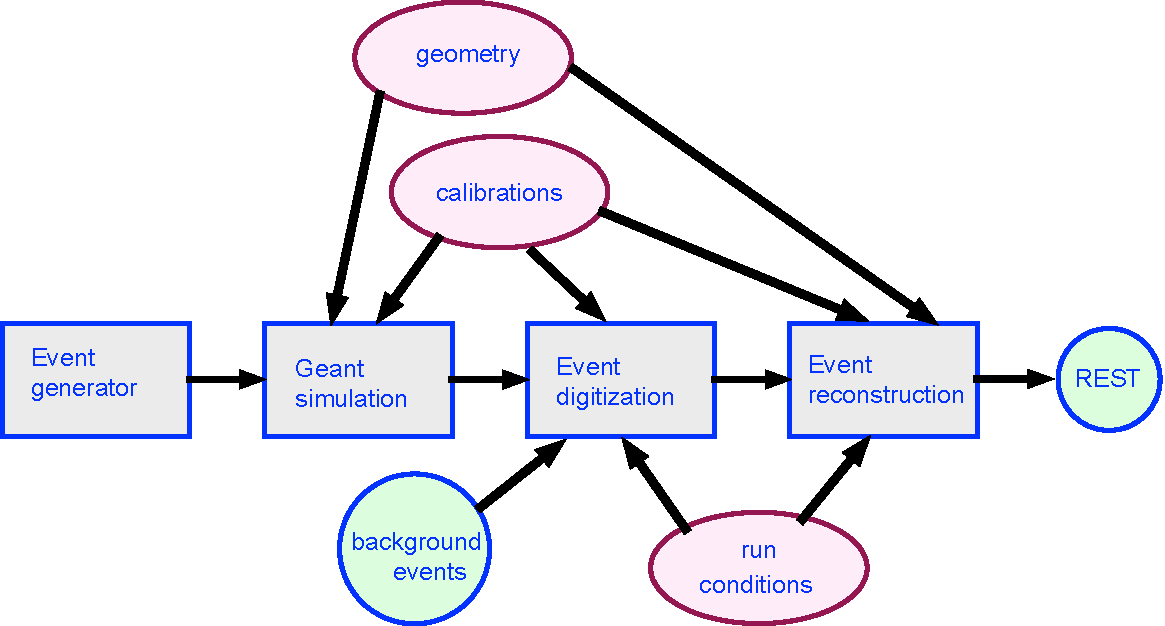
\includegraphics[width=0.85\textwidth]{figures/MC-data-flow.pdf}
\caption[]{\label{fig:MC-data-flow}The data flow from event generator through physics analysis files for Monte Carlo events.}
\end{figure}
\subsubsection[Material thickness]{\label{sec:materialscan}Geometry definitions}
The geometry and material descriptions for the experiment are common across simulation and reconstruction. The primary description resides in a family of xml files which all follow a common dtd or schema called the Hall D Detector Specification, or HDDS \textcolor{blue}{CITATION??}. Run-specific variations to this description are maintained in the Calibration Database, including information on missing and problematic electronic channels. The common magnetic field map is also maintained in the calibration database.

\subsection{Event generators \label{sec:generators}}
Simulation starts with the generation of events, which can be specific particles or reactions, or a background generator. A common tool set has been developed to minimize redundancy in code. These tools include standard methods to generate the distributions of primary photon beam energies and polarization. An output interface to produce files suitable as input for Geant simulation.

The photon beam energy distribution can be produced using a coherent bremsstrahlung generator that accounts for the physical properties of the radiator and the photon beamline.This generator also allows the user to select the orientation of the diamond radiator and then calculates the linear polarization for each photon. Photons can also be generated according to the spectrum measured in the pair spectrometer during any actual data run by interfacing to the calibration data base. In this method, the user inputs the degree of linear polarization and the orientation. Finally, the user can provide a histogram of the photon energy spectrum and a second one of the degree of polarization that is used to generate the photon beam. 

One of the first generators has been used to simulate the entire photoproduction cross section and is used to study backgrounds to physics reactions as well as develop analysis tools for extracting signals. This is based on Pythia~\cite{Sjostrand:2006za}, but includes additions that describe the low-energy photoproduction cross sections. Other generators are tied to specific reactions, where the generator needs to describe the underlying physics

\subsection{HDGeant \label{sec:hdgeant}}
As noted earlier, both Geant3 and Geant4 versions are available for simulation of the experiment. Both versions have been tuned to reproduce the behavior of the experiment, but there are some differences due to differences in how the two versions of Geant decide when to stop tracking particles. In general, simulation is carried to mimic the running conditions found across a range of runs; typically a large part of a single run period. The output from Geant is both hit time and energy deposits in detector volumes. 

\subsection[mcsmear]{Detector Response}
Converting the time and energy deposits coming from Geant into electronic detector responses that match what is readout from the experiment is carried out by the detector response package (mcsmear). The output of this digitization is identical to the real data with the exception that the so-called \emph{truth information} about the data is retained to allow detailed performance studies. In addition to the digitization, it is at this stage that run-dependent efficiency effects are applied to the data. This includes both missing electronic channels, as well as reduced efficiency of other channels. Additional smearing of some signals is also applied here to better match the performance of the Monte Carlo to data. 

In addition to the digitization, this package also folds measured backgrounds into the data stream. During regular data collection, random triggers are collected on a regular basis during each run. These are separated from the actual data and used to provide experimental background signals in the Monte Carlo, with rate of random events added based on the actual beam fluxes in the experiment. 

\subsection{Job submission \label{sec:jobsubmission}}
Because of the large number of experimental conditions that need to be matched in simulating data, the \emph{MCWrapper} tool has been developed to manage simulations. The tool can be used 'stand-alone' and integrates with various GlueX databases to allow users to run their own individual Monte Carlo workflows in sets of experimental runs with parameters of those runs automatically used.  MCwrapper also provides Monte Carlo samples in proportion to the actual data taken.  In principle this should better model the differences between runs and provide a simulated data set more comparable to the data.  Users who need a Monte Carlo sample can also use a web-based interface (Figure \ref{fig:MCWrapperSubmit} to MCWrapper (MCWrapper-bot) to select the event generator, the version of Geant, the run period of interest and versions of reconstruction and simulation code. This form is dynamic and only presents options to users as needed.  This keep clutter to a minimum and reduces potential confusion when approaching simulation in GlueX. Incorporated into the web form is also a simple web form to properly configure the analysis of produced files from the reconstruction step.  This is done in plain-text as to reduce errors in configuration. Once submitted MCWrapper-bot then correctly configures MCWrapper based on information provided by the user.  Once configured the automated system tests a small sub-sample of the request with the requested software stack.  This attempts to limit flawed submissions to computational resources.  On test failure the submitting user is supplied all logging information and a link that allows them to correct any miss-configuration and flag their project to be retested.  All of this happens without user intervention.  When the test is passed the system breaks the request into a number of jobs and submits the needed jobs to one of several systems.  The primary system used is the Open Science Grid, however the system decides on where to submit the job on a job by job basis. For example, if the system detects a forming backlog on the Open Science Grid, marked in part by a large number of idle jobs, it will seamlessly begin submitting to the local Jefferson Lab computing farm. While running all aspects of the requests and jobs are monitored.  If a job encounters problems MCWrapper-bot will attempt to diagnose it and may even take corrective action automatically (e.g. resubmitting failed jobs that fail for transient reasons). Once completed the system checks for expected files to be returned.  If expected files are not found the system will automatically submit a replacement job. Once the jobs are verified completed and all data from the request has been properly moved, the user receives an automated email alerting them to the fact that their request has been fulfilled and the location where the user can access the event sample.\newline
Users are able to monitor projects as well as control their projects via an online dashboard (Figure \ref{fig:MCWrapperDashboard}).  The MCWrapper dashboard gives information about active projects and allows users (or administrators) to interact with their requests by right-clicking on the individual row.  Users may cancel, suspend, or declare projects complete. By left-clicking on a row more detailed information is presented including the individual jobs, where the jobs are being run, basic usage statistics of the jobs, and current status.  Users may also see news or notices of outages regarding MCWrapper-bot.  These news articles are dynamically pushed to people on the web page and do not require a browser refresh to obtain.  Not shown are plots of the total number of running and idle jobs from the submit node (a measure of the health and load of the system). Also not shown are the heart beats of the subsystems of MCWrapper-bot with the system the last job was submitted to.  All information on the dashboard is dynamically updated in near real-time.  This gives individuals a near real-time look into the production of their Monte Carlo samples.
\begin{figure}[h!]\centering
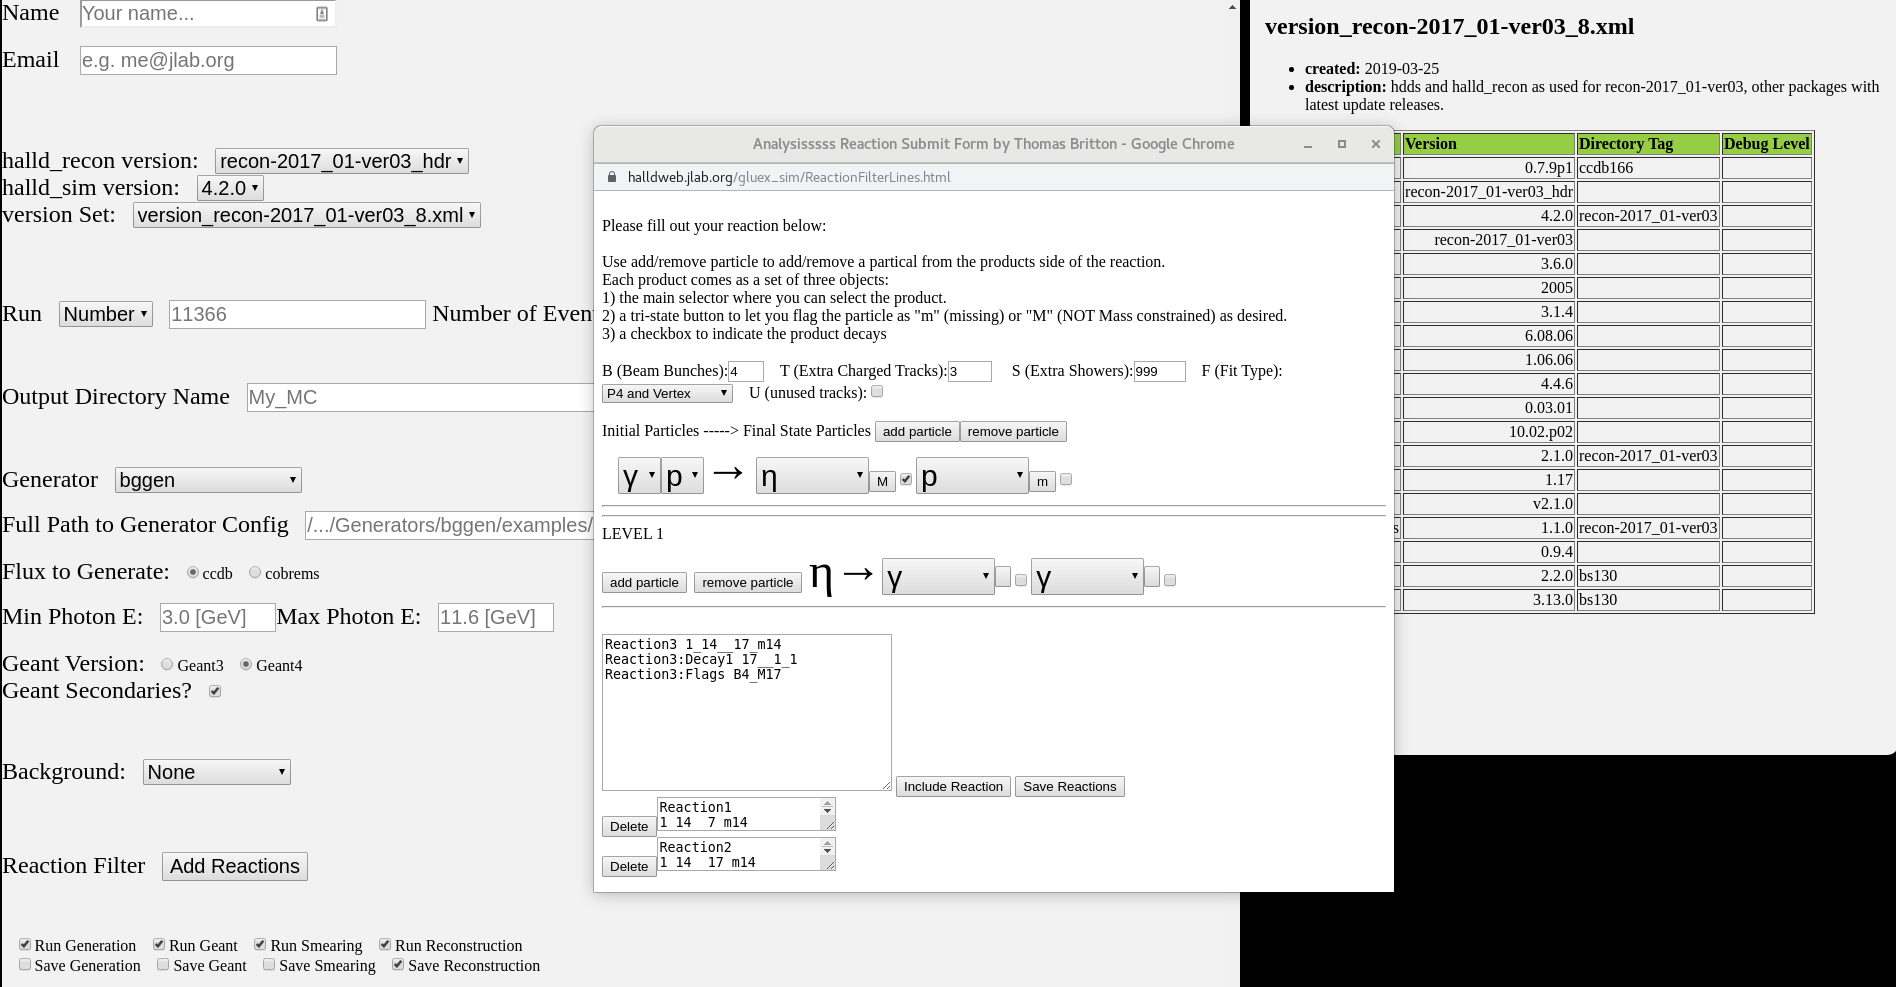
\includegraphics[width=0.85\textwidth]{figures/mcwrapper_submit_form.png}
\caption{Shown is a section of the web interface where users can request the various configuration parameters including the desired reactions to be analyzed.  The form dynamically generates options as needed}{\label{fig:MCWrapperSubmit}}
\end{figure}
\begin{figure}[h!]\centering
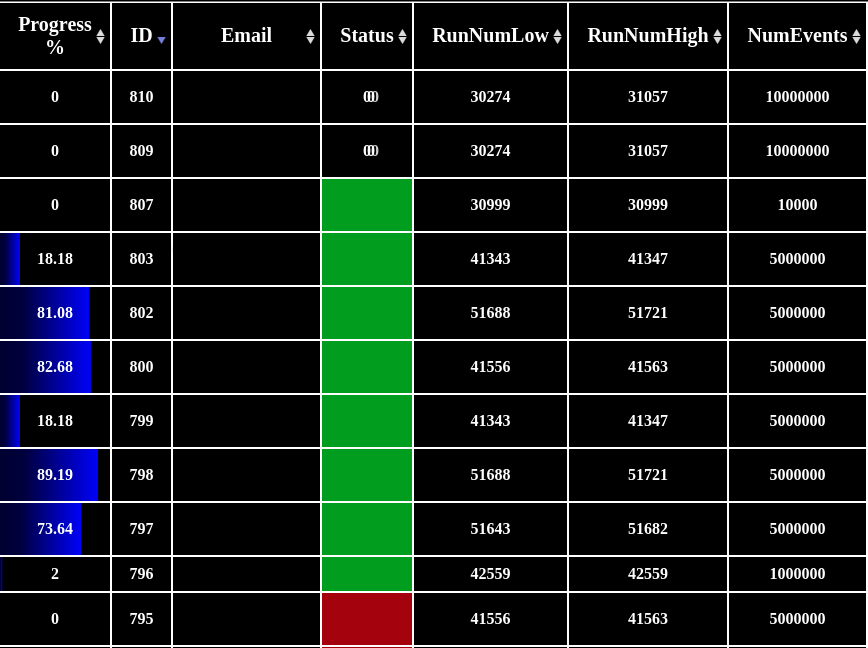
\includegraphics[width=0.85\textwidth]{figures/mcwrapper_dashboard_redacted.png}
\caption{Shown is a section of the main table of the MCWrapper dashboard with user email addresses redacted. The table provides useful information to users including the current level of completion, the status of the project (green for successfully tested, red for failed tests, and animated ellipses for project currently in testing).  }{\label{fig:MCWrapperDashboard}}
\end{figure}